\documentclass[14pt]{extarticle}
\usepackage[utf8]{inputenc}
\usepackage{ngerman}
\usepackage{array}
\usepackage{amsmath}
\usepackage{graphicx}
\title{Bericht Todesstern U5 - Transformationen}
\author{Charline Waldrich, Robert Ullmann, Julian Dobrot}
\date{15. Dezember 2015}

\begin{document}

\maketitle
\pagebreak
\tableofcontents

\section{Aufgabenstellung}
Implementierung von Samplings im Raytracer. Es soll zunächst ein Sampling Pattern erzeugt werden können, wobei di Punkte in einem regelmäßigen Raster angeordnet sind. Die Anzahl der Zeilen und Spalten können angegeben werden. Die Camera hat als weiteren Parameter ein Sampling Pattern. Die Methode rayRor gibt nicht länger einen einzelnen Strahl sondern eine Menge von Strahlen für einen Pixel zurück. Um die Farbe eines Pixels zu berechnen wird zunächst die Farbe für jeden Strahl ermittelt. Der Durchschnitt aller Werte genommen und dem Pixel zugewiesen. 
\subsection{Lösungsstrategien}
Übernehmen der Klassen Point2, Sampling Pattern aus dem UML Diagramm der Aufgabenstellung. 


\subsubsection{Implementierung}



\subsection{Probleme und besondere Ereignisse}


\subsection{Tests}
Die Abbildung zeigt die Transformierte Kugel aus der Aufgabenstellung.\\\\
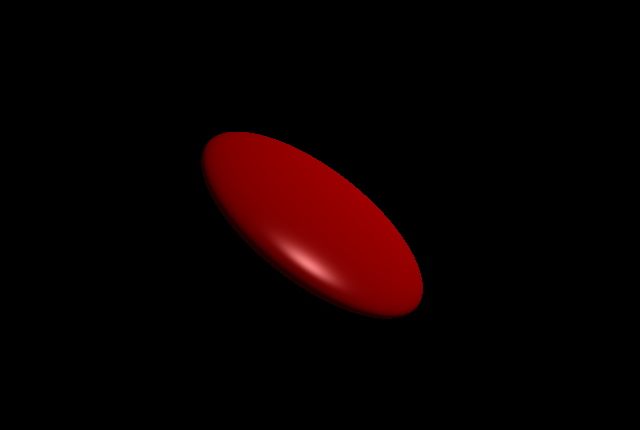
\includegraphics[width=10cm,height=10cm]{images/tr_abb_1}\\\\\\\\\\
Die Abbildung zeigt die Transformierte AAB aus der Aufgabenstellung.\\\\
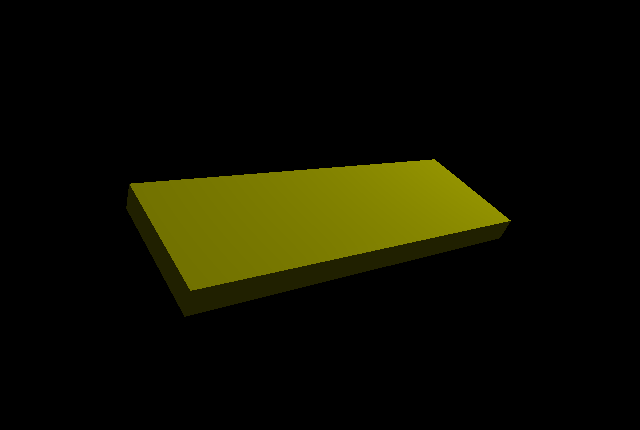
\includegraphics[width=10cm,height=10cm]{images/tr_abb_2}\\

\section{Zeitbedarf}
\begin{center}
\begin{tabular}{cr}
Änderungen an bestehenden Klassen \	&60 min	\\
UML Diagramm	  \	&100 min	\\
Implementiereung 	\	&180 min	\\
Programmierung \	&300 min	\\
Umstellung \	&120 min	\\
Bericht  \		&100 min	 \\
	\hline
	&860 min
\end{tabular}
\end{center}

\section{Quellen}

\end{document}
